\section{Datenbank und Datenmodell}

Da das Datenmodell einer Datenquelle Listen von anderen Datenmodell enthält, bietet sich hier als einfachste Lösung die Verwendung einer dokument-orientierten NoSQl-Datenbank an.
Das hat den Vorteil, dass diese Listen direkt in den Objekten der Datenquellen abgelegt werden können.
In Datenbanken, die Tabellen verwenden, müsste man für jedes Modell eine eigene Tabelle erstellen und die Verknüpfungen über über JOIN-Operationen auflösen.
Bei jeder Abfrage einer Datenquelle aber auch die verknüpften Einträge der Ingestion-Events oder Revisionen gebraucht werden.
Außerdem gibt es viele Anfragen auf die Datenquellen, da diese nicht zwischen den Mircoservices ausgetauscht werden und so nicht im Speicher vom Service verwaltet werden können.
Daher ist es effizienter die relevanten Daten direkt mit einer Abfrage laden zu können.
Das Speichern der Felder für die Optionen beim Lesen und Schreiben wird auch dadurch erleichter, dass es kein Schema gibt.
Man kann so die Optionen einfach in einem Dokument in der Revision speichern.

Hier kommt \textit{MongoDB}\footnote{https://www.mongodb.com/} als Datenbank zum Einsatz.
\textit{MongoDB} kann frei verwendet werden und bei bei größeren Datenmengen verteilt eingesetzt werden.
\fref{fig:datamodel} zeigt einen Überblick, wie das entwickelte Datenmodell aus \ref{sec:datasourcemodel} gespeichert wird.

\begin{figure}
    \centering
    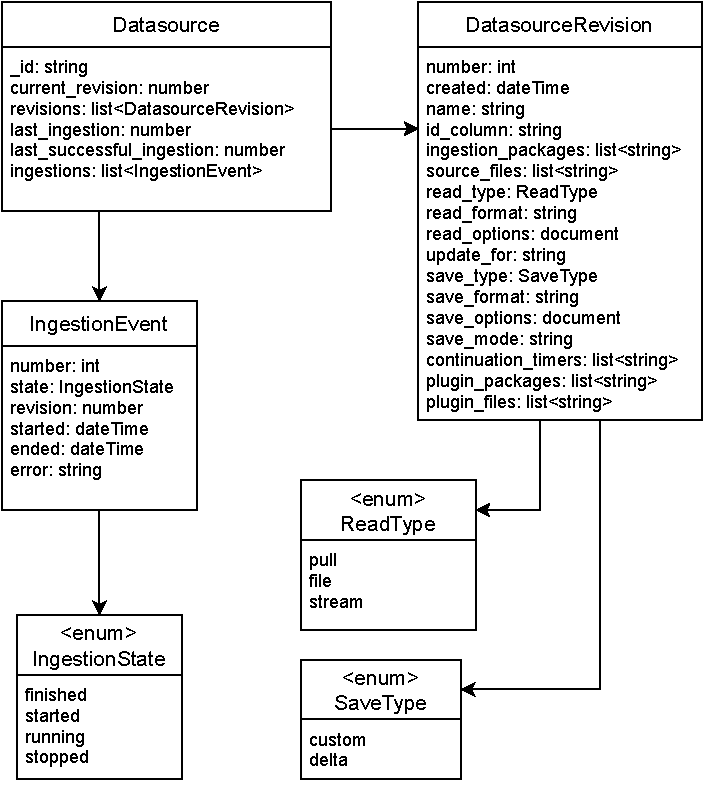
\includegraphics{Grafiken/ingestion-Datamodel.pdf}
    \caption{Übersicht Datenmodell}
    \label{fig:datamodel}
\end{figure}